\section{}
Fig. \ref{fig:Q1ProblemDiagram} shows a long, thing steel plate of thickness $t$, width $2h$, and length $2a$. The plate is
subjected to loads that produce the uniform stress $\sigma_o$ at the ends. The edges at $y=\pm h$ are placed between two 
rigid walls. Show that, by using an inverse method, the displacements are expressed by
\begin{equation*}
    u = - \frac{1-\nu^2}{E} \sigma_o x, \quad v = 0, \quad w = \frac{\nu (1+\nu)}{E} \sigma_o z
\end{equation*}

\begin{figure}[h]
    \centering
    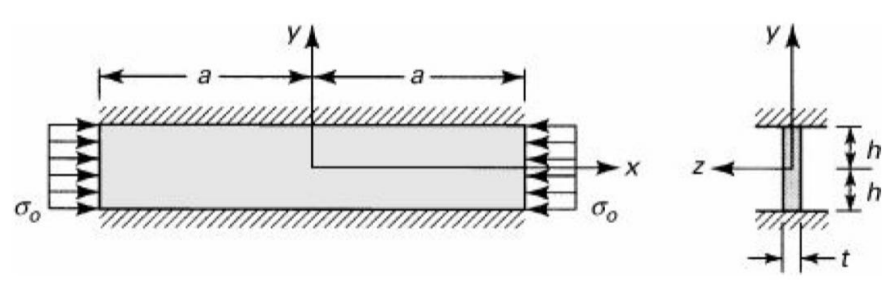
\includegraphics[width=0.5\linewidth]{Questions/Figures/Q1ProblemDiagram.png}
    \caption{Steel plate subjected to uniform stress $\sigma_o$ at the ends.}
    \label{fig:Q1ProblemDiagram}
\end{figure}
From the figure, $\sigma_x = -\sigma_o$ and $\sigma_z = 0$. The plane strain equations are
\begin{align*}
    \epsilon_x &= \frac{1}{E} \left( \sigma_x - \nu \sigma_y \right) \\
    \epsilon_y &= \frac{1}{E} \left( \sigma_y - \nu \sigma_x \right) \\
    \epsilon_z &= -\frac{1}{E} \left( \sigma_x + \sigma_y \right)
\end{align*}
Since there is a rigid wall at $y=\pm h$, $\epsilon_y = 0$. Therefore,
\begin{align*}
    \epsilon_y &= \frac{1}{E} \left( \sigma_y - \nu \sigma_x \right) \overset{\text{set}}{=} 0 \\
    \implies \sigma_y &= \nu \sigma_x= -\nu \sigma_o
\end{align*}
Also,
\begin{align*}
    \epsilon_y = \frac{\partial v}{\partial y} = 0 \implies \boxed{v = 0}
\end{align*}
From the $\epsilon_x$ equation,
\begin{align*}
    \epsilon_x &= \frac{1}{E} \left( \sigma_x -\nu \sigma_y \right) \\
    &= \frac{1}{E} \left( -\sigma_o - \nu (-\nu \sigma_o) \right) \\
    &= \frac{1}{E} \left( -\sigma_o + \nu^2 \sigma_o \right) \\
    &= \frac{1}{E} \left( \nu^2 - 1 \right) \sigma_o
\end{align*}
Since $\epsilon_x = \frac{\partial u}{\partial x}$, we can integrate to find $u$
\begin{align*}
    \epsilon_x &= \frac{\partial u}{\partial x} \\
    \implies u &= \boxed{\frac{1}{E} \left( \nu^2 - 1 \right) \sigma_o x}
\end{align*}
From the $\epsilon_z$ equation,
\begin{align*}
    \epsilon_z &= -\frac{1}{E} \left( \sigma_x + \sigma_y \right) \\
    &= -\frac{1}{E} \left( -\sigma_o - \nu \sigma_o \right) \\
    &= \frac{1}{E} \left(1 + \nu \right) \sigma_o
\end{align*}
Since $\epsilon_z = \frac{\partial w}{\partial z}$, we can integrate to find $w$
\begin{align*}
    \epsilon_z &= \frac{\partial w}{\partial z} \\
    \implies w &= \boxed{\frac{1}{E} \left(1 + \nu \right) \sigma_o z}
\end{align*}

